\documentclass{article}

\usepackage{../sty/notes}
\notenum{2}

\pgfplotsset{width=7cm}
\pgfplotsset{colormap={white}{color=(gray!20) color=(white)},
    colormap/white/.style={colormap name=white}}
\pgfplotsset{colormap={gray}{color=(gray) color=(gray!20)},
    colormap/gray/.style={colormap name=gray}}
\pgfplotsset{empty axes/.style={
    xtick=\empty,
    ytick=\empty,
    ztick=\empty,
    draw=gray}}
\pgfplotsset{white style/.style={
    surf,
    colormap/gray,
    mesh/interior colormap name=white,
    mesh/interior colormap thresh=0.05,
    samples=5, % 5 for fast rendering, 25 for accurate rendering
    domain=0:1}}


\begin{document}

\section*{Natural frequencies of floor slabs}

The natural stiffness of a floor slab can be approximated making use of the Rayleigh's method using an appropriate shape function satisfying the boundary conditions. From the static equilibrium equation of a slab, the modal mass and modal stiffness are rewritten according to the follwong expressions:
\begin{equation*}
\begin{aligned}
    m_\psi &= \int_0^{l_y}\int_0^{l_x} \rho t \psi^2 dxdy \\
    k_\psi &= \int_0^{l_y}\int_0^{l_x} D (\partial_{xx}\psi + \partial_{yy}\psi)^2 dxdy
\end{aligned}
\end{equation*}
where $\rho$ is the density, $t$ is the thickness and $D$ is the flexural stiffness, calculated from the Young's modulus $E$ and Poissins's ratio $\nu$ as
$$
D = \frac{Et^3}{12(1-\nu^2)}.
$$

\begin{wrapfigure}{l}{4cm}
\vspace{-1em}
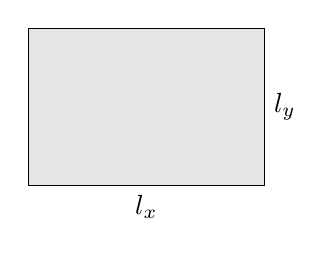
\begin{tikzpicture}
\draw [fill=gray!20] coordinate (O) rectangle (3,2) coordinate (P);
\path (O) -- node [midway,below] {$l_x$} (O -| P);
\path (O -| P) -- node [midway,right] {$l_y$} (P);
\end{tikzpicture}
\end{wrapfigure}

For a rectangular floor \emph{simply supported at the four sides}, the natural frequencies can be approximated using the following shape function, where $n$ and $m$ stand for the $i^\text{th}$ mode of vibration at the $x$ and $y$ directions,
$$
\psi = \sin\left(\frac{n\pi x}{l_x}\right) \sin\left(\frac{m\pi y}{l_y}\right).
$$
\\\vspace{1pt} % Enforce end of figure wrapping

The modal mass is
\begin{multline*}
m_\psi = 
\int_0^{l_y}\int_0^{l_x} \rho t \sin^2\left(\frac{n\pi nx}{l_x}\right) \sin^2\left(\frac{m\pi y}{l_y}\right) dxdy = \\
= \rho t \int_0^{l_x} \sin^2\left(\frac{n\pi x}{l_x}\right) dx \int_0^{l_y} \sin^2\left(\frac{m\pi y}{l_y}\right) dy =
\frac{\rho t l_x l_y}{4mn}.
\end{multline*}

The modal stiffness is
\begin{multline*}
k_\psi =
\int_0^{l_y}\int_0^{l_x}D \left[-\frac{n^2\pi^2}{l_x^2} \sin\left(\frac{n\pi x}{l_x}\right) \sin\left(\frac{m\pi y}{l_y}\right)\right.\\
\left.-\frac{m^2\pi^2}{l_y^2} \sin\left(\frac{n\pi x}{l_x}\right) \sin\left(\frac{m\pi y}{l_y}\right) \right]^2 dxdy = \\
= \pi^4D \left[ \frac{n^4}{l_x^4}\frac{l_x}{2n}\frac{l_y}{2m} + \frac{m^4}{l_y^4}\frac{l_x}{2n}\frac{l_y}{2m}
+ 2\frac{n^2m^2}{l_x^2l_y^2}\frac{l_x}{2n}\frac{l_y}{2m} \right] = \\
= \frac{\pi^4D}{4}\left(\frac{l_yn^3}{l_x^3m} + \frac{l_xm^3}{l_y^3m} + \frac{2mn}{l_xl_y}\right).
\end{multline*}

Finally, the frequencies of the slab are obtained after division of the above results,
\begin{align*}
\omega^2 &= \frac{k_\psi}{m_\psi} = \frac{\pi^4D}{4}\frac{4}{\rho t}
\left(\frac{n^4}{l_x^4} + \frac{m^4}{l_y^4} + 2\frac{n^2m^2}{l_x^2l_y^2}\right)
= \frac{\pi^4D}{\rho t}\left(\frac{n^2}{l_x^2} + \frac{m^2}{l_m^2}\right)^2 \\
\omega &= \pi^2\sqrt{\frac{D}{\rho t}} \left(\frac{n^2}{l_x^2} + \frac{m^2}{l_y^2}\right)^2
\end{align*}
and the first natural frequency is
\begin{equation*}
f_1 = \frac{\omega_1}{2\pi} = \frac{\pi}{2}\sqrt{\frac{D}{\rho t}} \left(\frac{1}{l_x^2} + \frac{1}{l_y^2}\right).
\end{equation*}


\begin{center}
    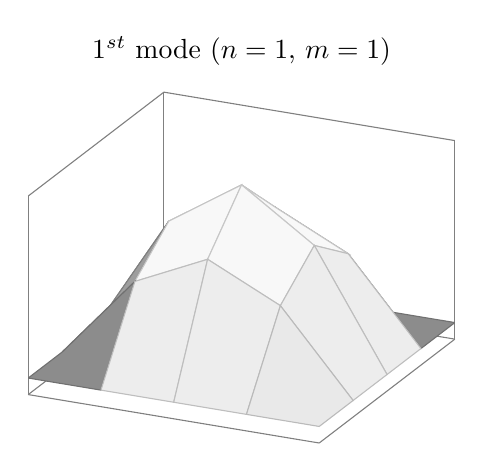
\begin{tikzpicture}
        \begin{axis}[empty axes,title={$1^\text{st}$ mode ($n=1$, $m=1$)}]
            \addplot3 [white style] {sin(180*x) * sin(180*y)};
        \end{axis}
    \end{tikzpicture}
    \hspace{1em}
    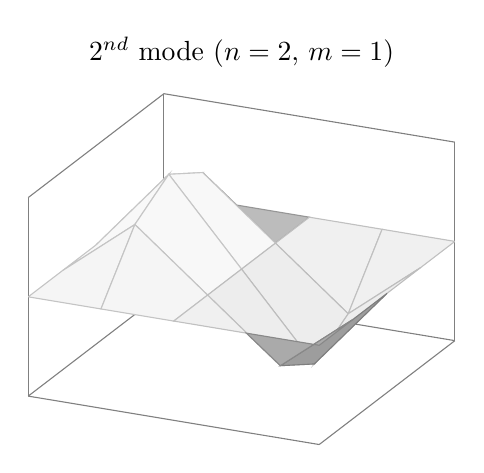
\begin{tikzpicture}
        \begin{axis}[empty axes,title={$2^\text{nd}$ mode ($n=2$, $m=1$)}]
            \addplot3 [white style] {sin(360*x) * sin(180*y)};
        \end{axis}
    \end{tikzpicture}
    
    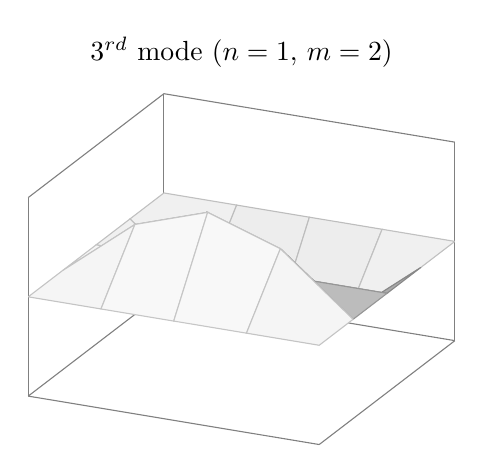
\begin{tikzpicture}
        \begin{axis}[empty axes,title={$3^\text{rd}$ mode ($n=1$, $m=2$)}]
            \addplot3 [white style] {sin(180*x) * sin(360*y)};
        \end{axis}
    \end{tikzpicture}
    \hspace{1em}
    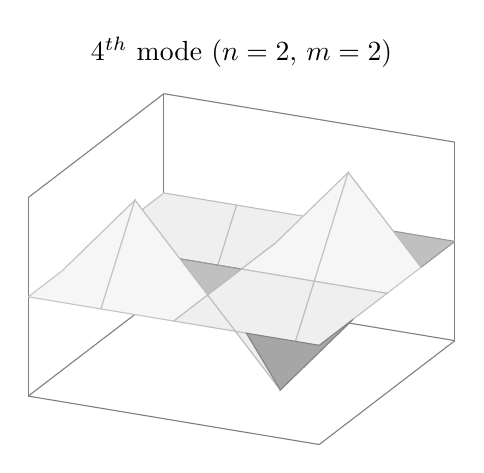
\begin{tikzpicture}
        \begin{axis}[empty axes,title={$4^\text{th}$ mode ($n=2$, $m=2$)}]
            \addplot3 [white style] {sin(360*x) * sin(360*y)};
        \end{axis}
    \end{tikzpicture}
\end{center}


\end{document}